\section{Техническое задание}
\subsection{Основание для разработки}

Основанием для разработки веб-приложения для сбора и анализа информации об инцидентах с общественным транспортом является задание на выпускную квалификационную работу приказ ректора ЮЗГУ от « » 2024 года № 0000-0 «Об утверждении тем выпускных квалификационных работ и руководителей выпускных квалификационных работ».


\subsection{Цель и назначение разработки}

Функциональное назначение разрабатываемого веб-приложения состоит в сборе, анализе и обработке информации, поступающей от пассажиров и граждан, касающейся инцидентов с общественным транспортом.
Оно направлено на устранение текущих недостатков, связанных с инцидентами в общественном транспорте.
 
 На данный момент приложение будет обрабатывать обращения, связанные с инцидентами в городском общественном транспорте безрельсового типа, такими как автобусы, маршрутные такси и троллейбусы. В будущем планируется увеличить масштаб функционала на все виды общественного транспорта.
 
Данное приложение позволит быстро и систематизировано обрабатывать инциденты, что поможет ответственным службам оперативнее реагировать на проблемы и минимизировать их влияние на пассажиров. Кроме того, приложение предоставляет гражданам платформу для обратной связи, способствуя повышению прозрачности и доверия к транспортным службам.

В соответствии с поставленной целью, были определены следующие задачи:
\begin{enumerate}
\item разработка информационного веб-приложения;
\item создание базы данных;
\item реализация функций авторизации и регистрации;
\item внедрение функционала для создания и отображения новостной ленты;
\item реализация системы обратной связи.
\end{enumerate}

В результате выполнения поставленных задач будет разработано полноценное информационное веб-приложение. Оно будет включать в себя надежную базу данных, обеспечивающую хранение, обработку и анализ информации, а также функции авторизации и регистрации пользователей. Дополнительно, приложение будет оснащено лентой новостей для своевременного информирования граждан и системой обратной связи, что позволит улучшить взаимодействие между пассажирами и другими участниками дорожного движения и транспортными службами.

\subsection{Требования пользователя к интерфейсу}

Веб-приложение должно содержать следующие компоненты:
\begin{itemize}
    \item форма регистрации;
    \item форма авторизации;
    \item форма для добавления обращения;
    \item раздел <<Новостная лента>>, представляющий собой список обращений, успешно прошедших модерацию;
    \item отображение рейтинга водителя;
    \item личный кабинет пользователя;
    \item административная панель.
\end{itemize}

На рисунках 2.1-2.4 представлены макеты интерфейса пользователя программного продукта.
\begin{figure}[H]
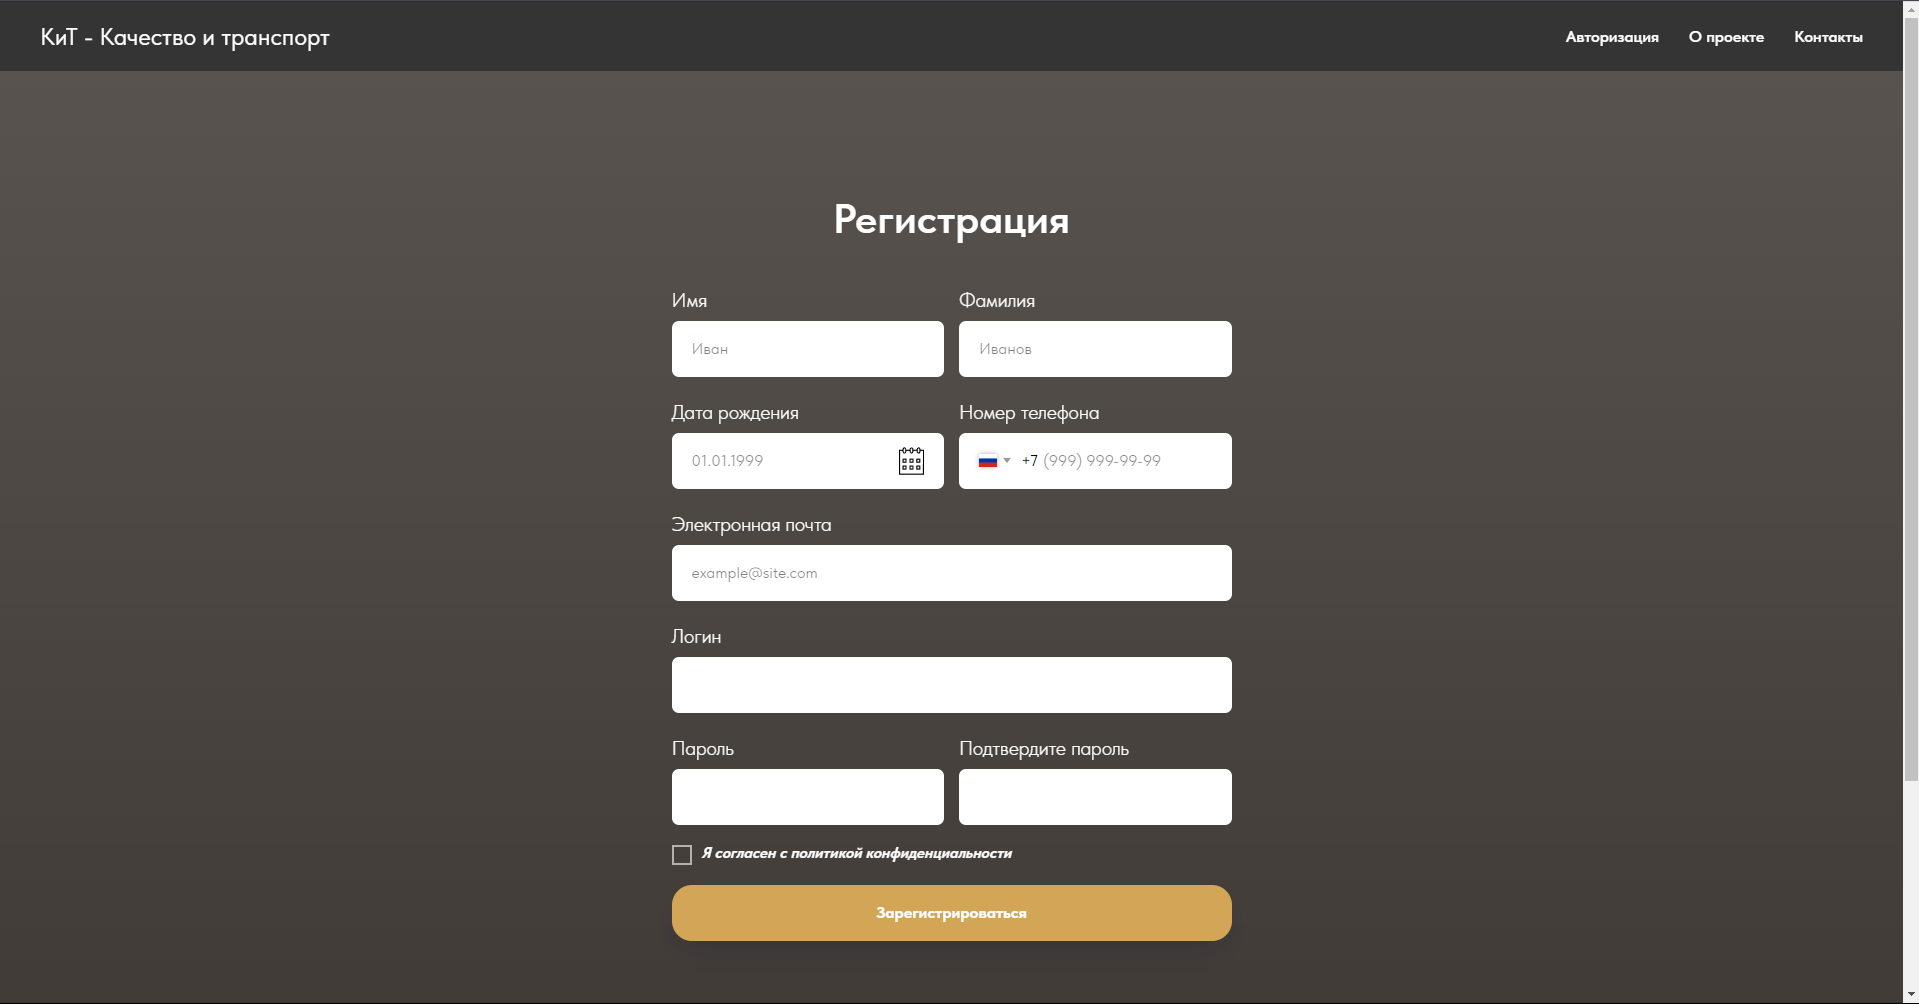
\includegraphics[width=1\linewidth]{Регистрация}
\caption{Макет формы регистрации}
\label{templ:image}
\end{figure}

\begin{figure}[H]
	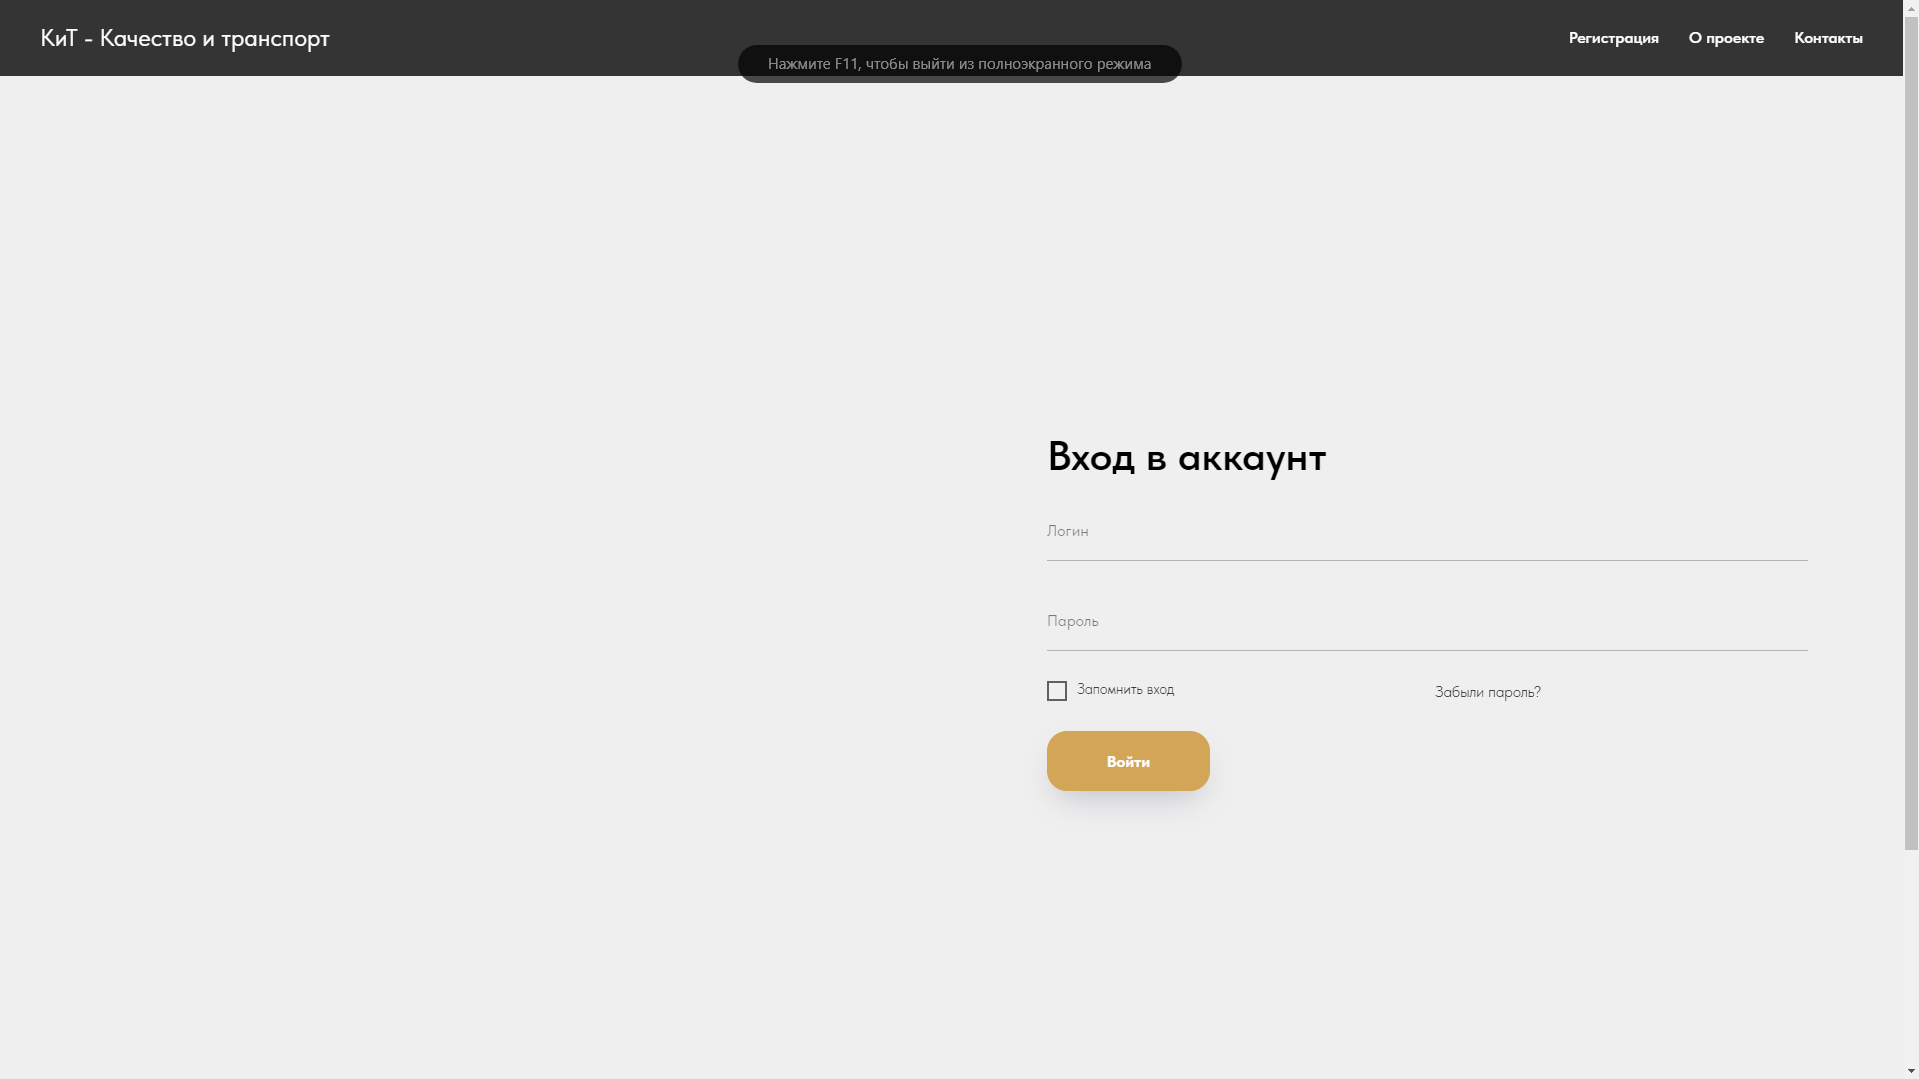
\includegraphics[width=1\linewidth]{Авторизация}
	\caption{Макет формы авторизации}
	\label{templ:image}
\end{figure}

\begin{figure}[H]
	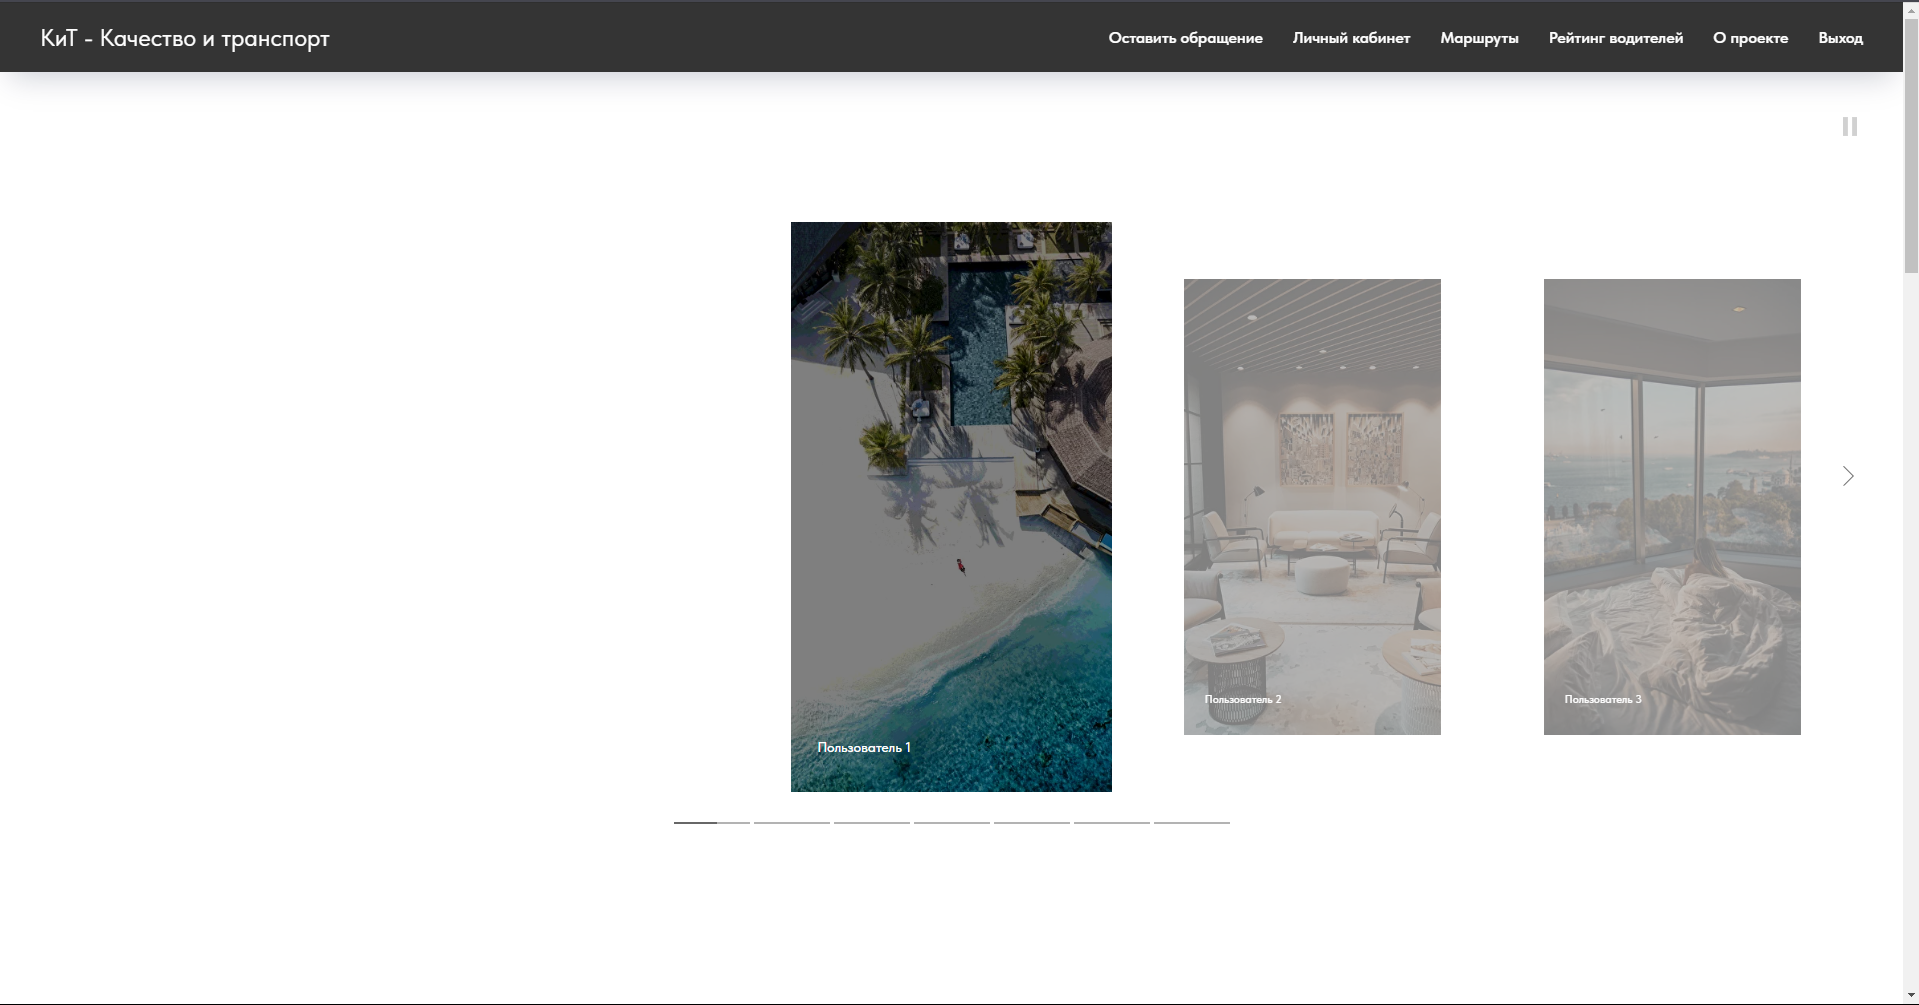
\includegraphics[width=1\linewidth]{Новостная лента}
	\caption{Раздел <<Новостная лента>>}
	\label{templ:image}
\end{figure}

\begin{figure}[H]
	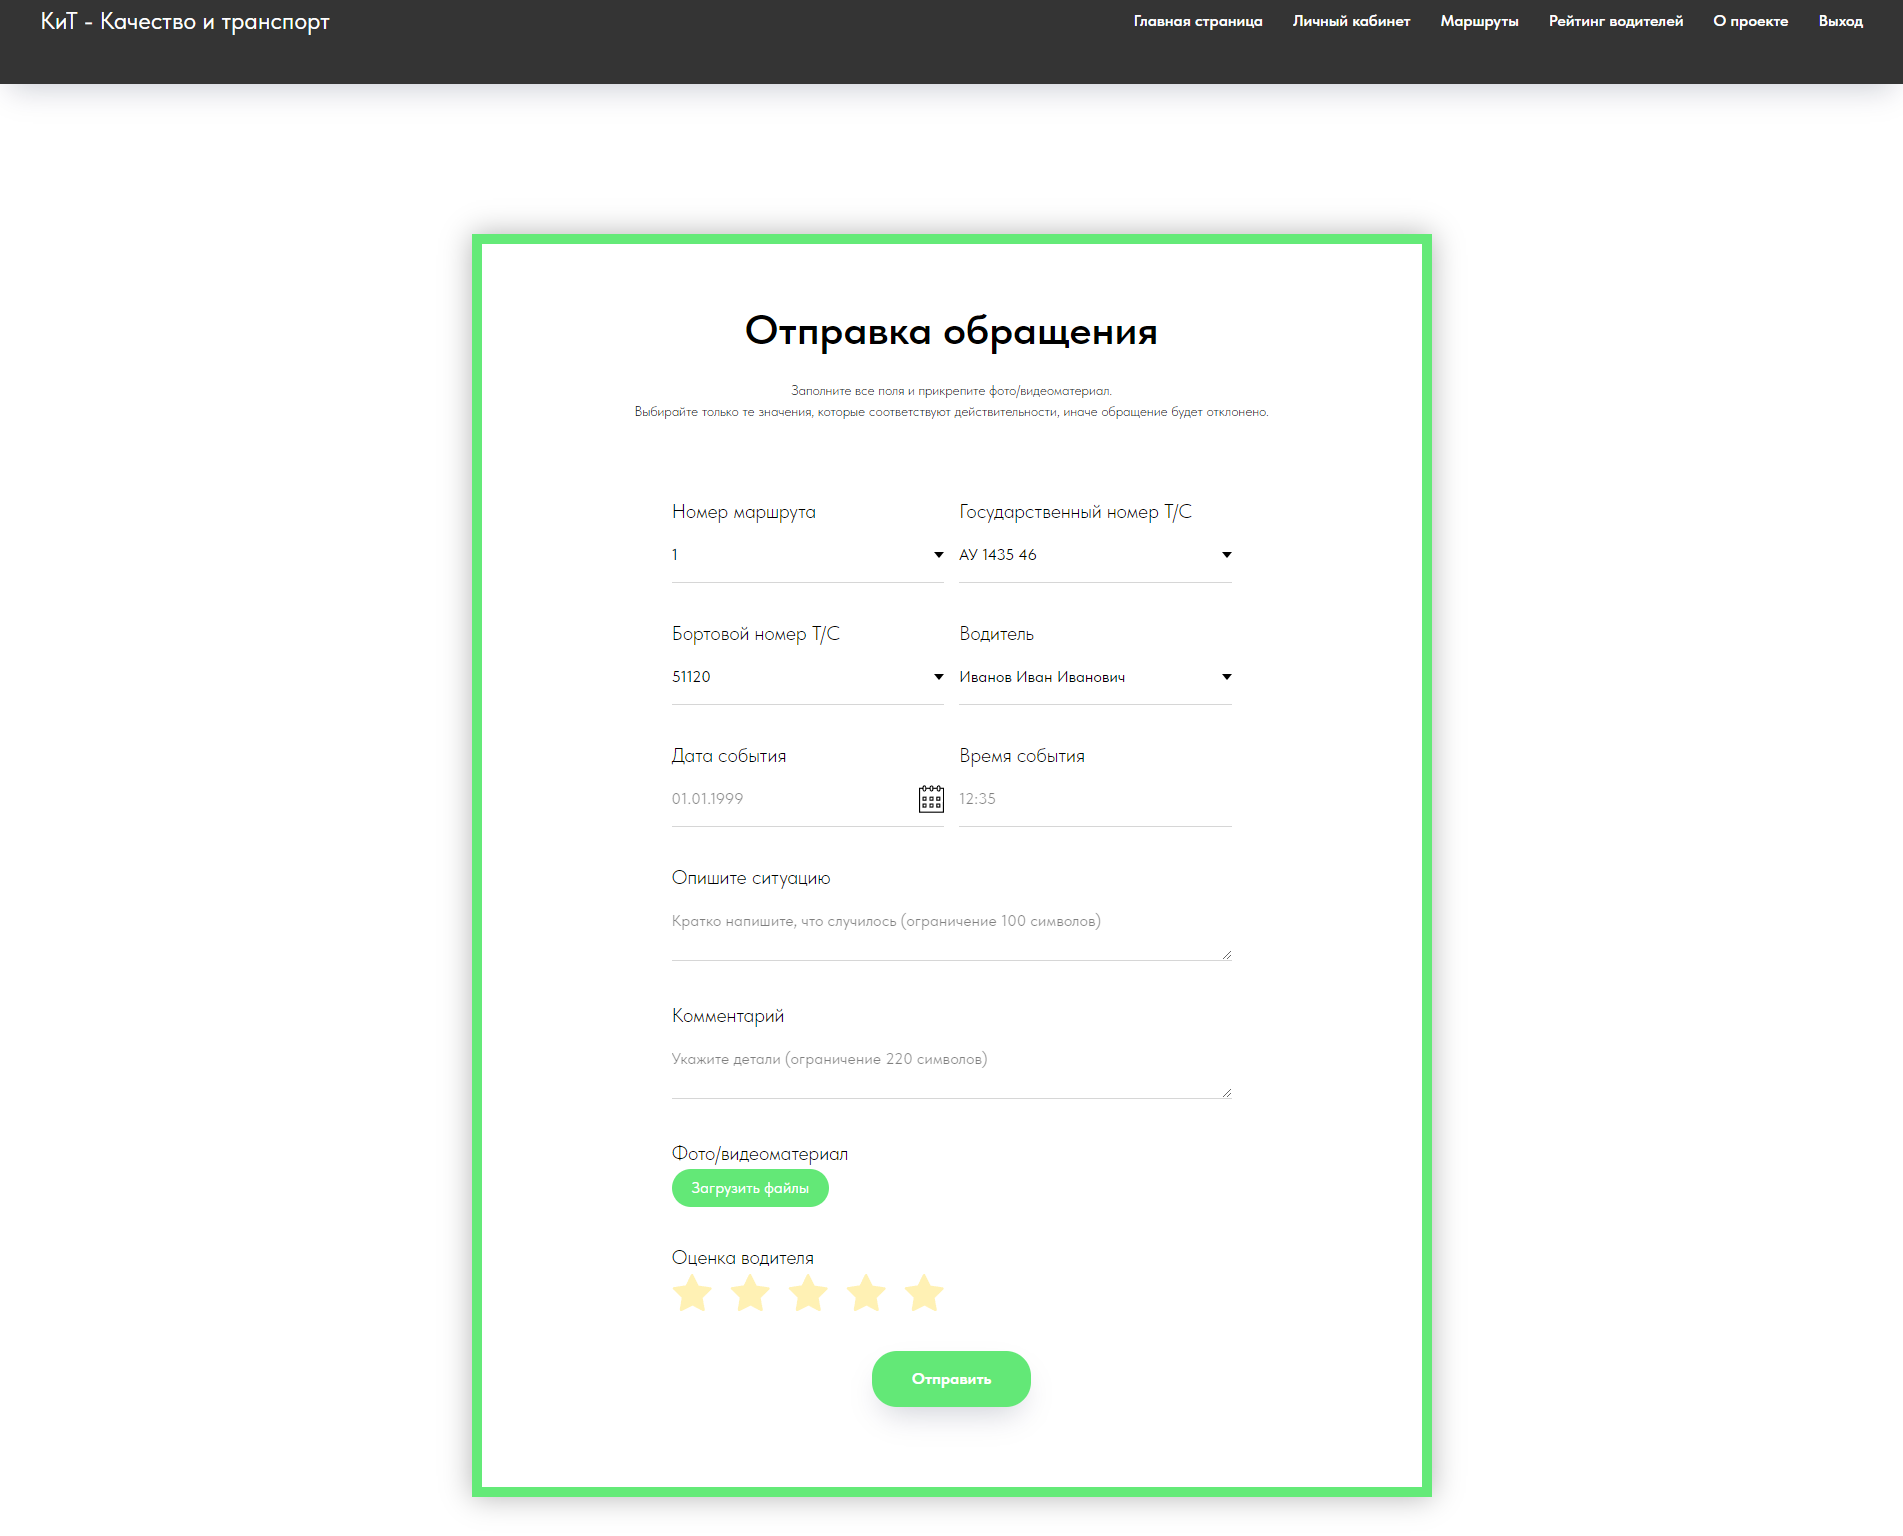
\includegraphics[width=1\linewidth]{Форма обращения}
	\caption{Раздел <<Отправка обращения>>}
	\label{templ:image}
\end{figure}

\subsection{Моделирование вариантов использования}

Для разрабатываемого веб-приложения была реализована диаграмма прецедентов - модель, обеспечивающая наглядное представление вариантов его использования. 

Она способствует физической разработке и детальному анализу взаимосвязей объектов. Для построения диаграммы вариантов использования применяется унифицированный язык визуального моделирования UML. 

Диаграмма вариантов использования описывает функциональное назначение разрабатываемой системы, то есть показывает, что система будет делать в процессе своего функционирования. Она представляет собой исходное концептуальное представление системы в процессе проектирования и разработки. В проектируемой системе прецеденты представляют собой действия, предоставляемые системой актерам или сущностям, взаимодействующим с системой. Актером является сущность, взаимодействующая с системой извне, будь то человек или техническое устройство. Прецедент описывает набор действий, которые система выполняет для актера.

На основании анализа предметной области в разрабатываемом веб-приложении сбора и анализа информации об инцидентах с общественным транспортом должны быть реализованы следующие прецеденты:
\begin{enumerate}
\item Регистрация аккаунта;
\item Авторизация пользователя;
\item Отправка обращений;
\item Публикация обращений;
\item Просмотр информации в личном кабинете;
\item Модерация обращений.
\end{enumerate}

На рисунке ~\ref{templ:image} представлены функциональные требования к системе в виде диаграммы прецедентов нотации UML.
\begin{figure}[H]
	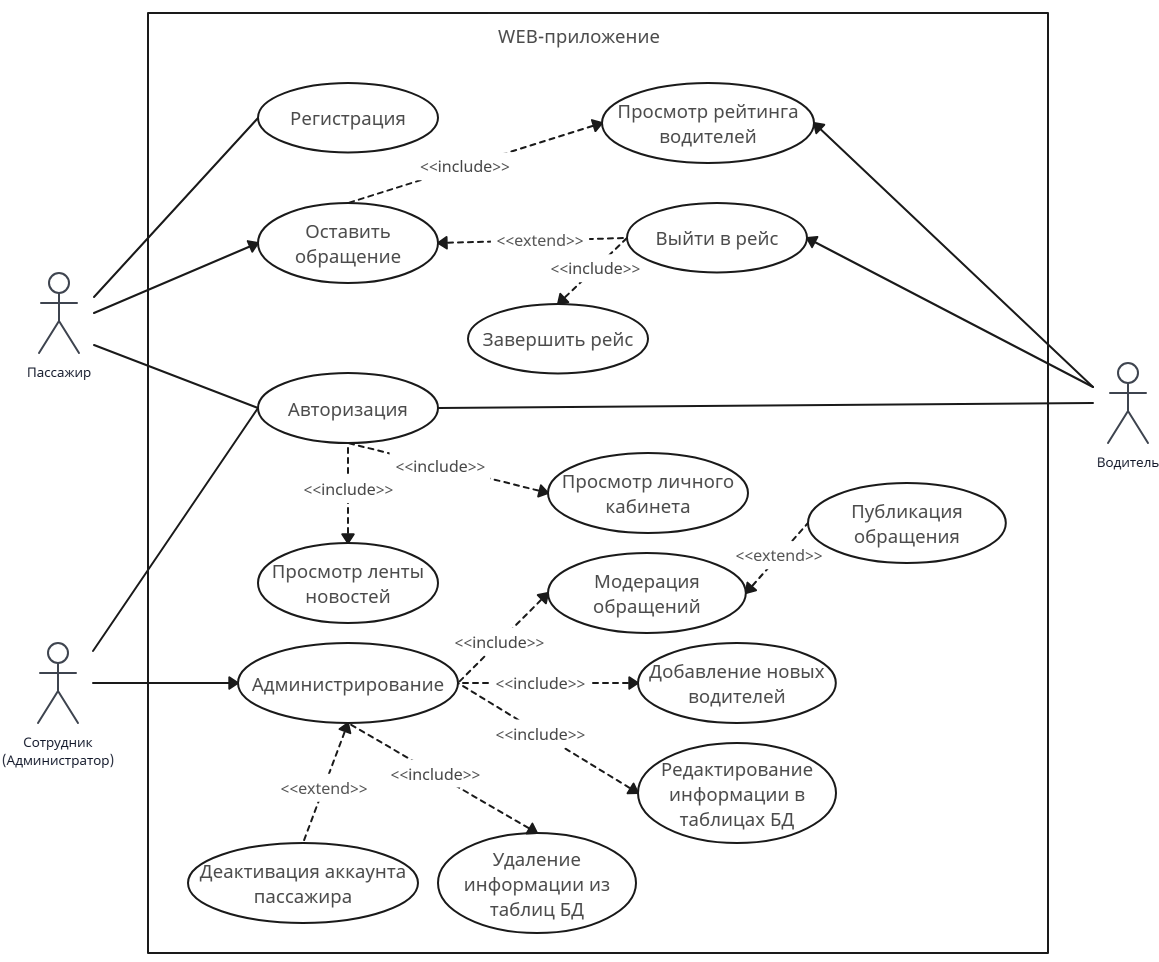
\includegraphics[width=1\linewidth]{Диаграмма прецедентов}
	\caption{Диаграмма прецедентов}
	\label{templ:image}
\end{figure}

\subsubsection {Вариант использования «Регистрация аккаунта»}
Заинтересованные лица и их требования: Пользователи, желающие получить доступ к веб-приложению.

Предусловие: Пользователь открывает страницу регистрации.

Постусловие: Пользователь имеет аккаунт в системе.

Основной успешный сценарий: 
\begin{enumerate}
\item Пользователь заходит на страницу регистрации.
\item Пользователь корректно заполняет все поля формы регистрации.
\item Пользователь нажимает на кнопку «Зарегистрироваться».
\item Система создает аккаунт пользователя.
\end{enumerate}

\subsubsection {Вариант использования «Авторизация пользователя»}
Заинтересованные лица и их требования: Пользователи, желающие получить доступ к веб-приложению.

Предусловие: Пользователь открывает страницу авторизации.

Постусловие: Пользователь попадает на главную страницу.

Основной успешный сценарий: 
\begin{enumerate}
	\item Пользователь заходит на страницу авторизации.
	\item Пользователь корректно вводит логин и пароль от своего аккаунта в соответствующих полях формы.
	\item Пользователь нажимает на кнопку «Войти».
	\item Система загружает главную страницу.
\end{enumerate}

\subsubsection {Вариант использования «Отправка обращений»}

Заинтересованные лица и их требования: Пользователи, желающие оставить обращение о случившемся инциденте.

Предусловие: Пользователь открывает раздел «Оставить обращение».

Постусловие: Пользователь отправляет обращение в систему.

Основной успешный сценарий: 

\begin{enumerate}
	\item Пользователь заходит в раздел «Оставить обращение».
	\item Пользователь заполняет все необходимые поля.
	\item Пользователь нажимает на кнопку «Отправить».
	\item Система создает новое обращение и отправляет его на проверку администратору.
\end{enumerate}

\subsubsection {Вариант использования «Модерация обращений»}

Заинтересованные лица и их требования: Пользователи, которые несут ответственность за корректность контента обращений.

Предусловие: Пользователь вошел в систему под своим аккаунтом, имеющим расширенные права доступа.

Постусловие: Пользователь допускает обращение для публикации.

Основной успешный сценарий: 

\begin{enumerate}
	\item Пользователь заходит в раздел «Новые обращения».
	\item Пользователь проверяет правильность введённых данных, а также содержание обращения на корректность и достоверность.
	\item Пользователь нажимает на кнопку «Опубликовать». 
	\item Система показывает обращение на главной странице с целью ознакомления для других пользователей.
\end{enumerate}

\subsubsection {Вариант использования «Просмотр информации в личном кабинете»}

Заинтересованные лица и их требования: Пользователи, желающие ознакомится или дополнить информацию о себе в личном кабинете.

Предусловие: Пользователь заходит в систему под своим аккаунтом. 

Постусловие: Пользователь просматривает или дополняет информацию о себе.

Основной успешный сценарий: 

\begin{enumerate}
	\item Пользователь заходит в раздел «Личный кабинет».
	\item Пользователь просматривает имеющуюся информацию и/или добавляет новую информацию.
	\item Пользователь нажимает на кнопку «Сохранить» при добавлении новых данных.
	\item Система выводит сообщение «Данные сохранены», при добавлении новых данных.
\end{enumerate}



\subsection{Требования к оформлению документации}

Разработка программной документации и программного изделия должна производиться согласно ГОСТ 19.102-77 и ГОСТ 34.601-90. Единая система программной документации.
